\documentclass[a4paper,12pt]{article}
\usepackage{fullpage}
\usepackage[british]{babel}
\usepackage{listings}

\usepackage{amsmath}
\usepackage{amssymb}
\usepackage{amsthm} \newtheorem{theorem}{Theorem}
\usepackage{color}
\usepackage{float}
\usepackage{listings}
\usepackage{subfig}
\lstset{% parameters for all code listings
	language=Python,
	frame=single,
	basicstyle=\small,  % nothing smaller than \footnotesize, please
	tabsize=2,
	numbers=left,
	framexleftmargin=2em,  % extend frame to include line numbers
	%xrightmargin=2em,  % extra space to fit 79 characters
	breaklines=true,
	breakatwhitespace=true,
	prebreak={/},
	captionpos=b,
	columns=fullflexible,
	escapeinside={\#*}{\^^M}
}

% Alter some LaTeX defaults for better treatment of figures:
    % See p.105 of "TeX Unbound" for suggested values.
    % See pp. 199-200 of Lamport's "LaTeX" book for details.
    %   General parameters, for ALL pages:
    \renewcommand{\topfraction}{0.9}	% max fraction of floats at top
    \renewcommand{\bottomfraction}{0.8}	% max fraction of floats at bottom
    %   Parameters for TEXT pages (not float pages):
    \setcounter{topnumber}{2}
    \setcounter{bottomnumber}{2}
    \setcounter{totalnumber}{4}     % 2 may work better
    \setcounter{dbltopnumber}{2}    % for 2-column pages
    \renewcommand{\dbltopfraction}{0.9}	% fit big float above 2-col. text
    \renewcommand{\textfraction}{0.07}	% allow minimal text w. figs
    %   Parameters for FLOAT pages (not text pages):
    \renewcommand{\floatpagefraction}{0.7}	% require fuller float pages
	% N.B.: floatpagefraction MUST be less than topfraction !!
    \renewcommand{\dblfloatpagefraction}{0.7}	% require fuller float pages

	% remember to use [htp] or [htpb] for placement


\usepackage{fancyvrb}
\DefineVerbatimEnvironment{code}{Verbatim}{fontsize=\small}
\DefineVerbatimEnvironment{example}{Verbatim}{fontsize=\small}

\usepackage{tikz} \usetikzlibrary{trees}
\usepackage{hyperref}  % should always be the last package

% useful colours (use sparingly!):
\newcommand{\blue}[1]{{\color{blue}#1}}
\newcommand{\green}[1]{{\color{green}#1}}
\newcommand{\red}[1]{{\color{red}#1}}

% useful wrappers for algorithmic/Python notation:
\newcommand{\length}[1]{\text{len}(#1)}
\newcommand{\twodots}{\mathinner{\ldotp\ldotp}}  % taken from clrscode3e.sty
\newcommand{\Oh}[1]{\mathcal{O}\left(#1\right)}

% useful (wrappers for) math symbols:
\newcommand{\Cardinality}[1]{\left\lvert#1\right\rvert}
%\newcommand{\Cardinality}[1]{\##1}
\newcommand{\Ceiling}[1]{\left\lceil#1\right\rceil}
\newcommand{\Floor}[1]{\left\lfloor#1\right\rfloor}
\newcommand{\Iff}{\Leftrightarrow}
\newcommand{\Implies}{\Rightarrow}
\newcommand{\Intersect}{\cap}
\newcommand{\Sequence}[1]{\left[#1\right]}
\newcommand{\Set}[1]{\left\{#1\right\}}
\newcommand{\SetComp}[2]{\Set{#1\SuchThat#2}}
\newcommand{\SuchThat}{\mid}
\newcommand{\Tuple}[1]{\langle#1\rangle}
\newcommand{\Union}{\cup}
\usetikzlibrary{positioning,shapes,shadows,arrows}


\title{\textbf{Evolutionary Simulator In A Dynamic Environment}}

\author{Jonathan Sharyari \and Lukas Klingsbo}  % replace by your name(s)

%\date{Month Day, Year}
\date{\today}

\begin{document}

\maketitle

\section*{Abstract}
Genetic algorithms (GAs) are a well established optimization tool for static problems. Recently, genetic algorithms have been proposed to improve the adaptivity of GAs in dynamic environments. In this paper, we attempted to implement and compare some of these methods; two methods based on mutation, and two based on periodic insertions of \emph{immigrants}. A extensive and easily available test environment was developed and used in order to compare the performance of these methods. The results show that the immigrant-based methods were useful for some types of  dynamic systems.


\section{Introduction}
Genetic algorithms are a common tool to find solutions to complex problems, often with high dimensionality. Although much research has been done on the subject, this research has to some extent focused on problems in a stationary environment.

Since in a dynamic environment the fitness conditions are changing over time, a traditional GA is not very suited for solving dynamic problems, as it is likely that the population will quickly converge and not be able to adapt when the environment changes.

Several approaches have been proposed in order to allow GAs to maintain the population diversity, two common methods are \emph{random} or \emph{elite immigrants} and \emph{triggered hypermutation} [1][2].

The goal of this project is to evaluate the methods proposed in earlier work, on a dynamic environment designed for the purpose.

\section{Environment}
Our test environment consists of a simple map containing clusters of "food", and is initialized randomly. The goal of the population is to find paths leading to areas where the food is distributed. A dynamic environment is created by changing the positions of the food in the map. This can be done in many ways, and we settle for three different methods of changing the map.

\begin{itemize}

\item
Slightly changing - Small changes are done, but fairly often. The optimum after a change will lie close to the earlier optimum.
\item
Abruptly changing - The map is reinitialized, changing the positions of obstacles and enemies. This must be done rarely, as to give the population the time to re-adapt.
\item
Seasonally changing - similar to abrupt changes, the changes are large and rare, but the number of maps is finite and periodic.
\end{itemize}

We anticipate that the different dynamic methods tested (explained below) will perform differently depending on the type of dynamic maps used.

\section{Suggested Dynamic Methods}
\subsection{Hypermutation}
The concept of mutation is critical for genetic algorithms, as it is through mutation a genetic algorithm maintains its diversity. As the problem of training in a dynamic environment is to avoid or overcome early convergence, it is tempting to try training with a higher degree of mutation than commonly used in static environments. Although this is a simple concept, \cite{cobb} shows that this method can generate relatively good results.

\subsection{Triggered Hypermutation}
A higher mutation rate results in higher diversity as indicated above, but a high mutation rate makes it more difficult to converge. The mutation rate is therefore generally kept low in standard GAs. The method of using a high mutation rate in a dynamic system might therefore lead to non-converging individuals.

Triggered hypermutation is a proposed solution to this problem. The mutation rate in general is kept low, giving better convergence. When the system is altered in a way that decreases the fitness, the hypermutation stage is started and the mutation rate is temporarily increased giving the same effect as the method explained above, but hopefully avoids the negative effects.

The results in \cite{cobb} and \cite{simoes} show that this method is efficient when the changes in the environment are small, but does not cope as well with abrupt changes.


\subsection{Immigrants}
Random immigrants and elitism-based immigrants use a different approach to maintain diversity. In these methods, some individuals with low fitness are removed and replaced with new individuals.

With random immigrants, these new individuals are randomly created (by the same method individuals were initialized at the beginning).

With elitism-based immigrants, the individuals with high fitness are remembered. When the total fitness decreases (potentially due to changes in the environment), individuals with low fitness are removed and individuals from this elite-set are reintroduced.

The random immigrants method has been shown to be beneficial for most dynamic environments, compared to the standard GA, but not necessarily the best method\cite{yang}. Using elite immigrants, the results can be improved for slightly changing and seasonal environments, but as this method keeps a lower diversity, it does not perform as well when the changes are more abrupt.

\section{Genome representation}
The behavior of an individual depends on its genome, which decides how it moves on the map. The genome is represented as a matrix of vector values where each position in the matrix represents a part of the map, and the vector stored at the position is the direction in which the individual will move. For a matrix of size $m \times n$, this is represented as m arrays of size n.

Consider a map of size $50m \times 50n$ and a matrix of size $m \times n$. Then every matrix position will represent a $50\times50$ square in the map. When the individual has a position inside that square, it's speed and direction will be given by the vector stored in that position of the matrix.

\section{Selection and Crossover strategies}
Two different crossover types were used, epoch and collision learning. In collision learning, the individuals crossover when they collide in the map, provided they have collected some fixed amount of food. Two new individuals are created by one either one-point, two-point or uniform crossover.

This type of crossover was useful during implementation, as the results could easily be seen graphically. But as this is not a traditional way of selection, epoch learning was used as only then could the implementation of the above methods be done in a way that is comparable with the result in previous research.

In epoch learning, the individuals search the map for a fixed set of updates, one epoch. At the end of the epoch, individuals were re-combinated and mutated depending on the settings used. The selection method used worked by first sorting the list of individuals, with the highest fitness first, using the number of food collected as a measure of the fitness. Then, each individual from the beginning crosses over with a probability $\alpha$ with the first individual. If not, the individual crosses over with the same probability $\alpha$ with the second individual, and so on. In general, only the best half of the individuals reproduce.

\section{Results}
During the course of this project, the above proposed algorithms were implemented and testing was performed in order to compare their performances. To this effect, tests were run for all combinations of maps (static, slightly changing, abruptly changing and periodicly changing maps) and every algorithm (normal, high mutation, triggered hypermutation, random immigrants, elite immigrants).

In order to perform testing, a graphical web-interface was created. This interface can for a limited time be reached at http://mindlevel.net. As to keep the differences between how the algorithms were tested as low as possible, most parameters were kept constant during testing;

\begin{lstlisting}
Training: epoch
Individuals: 15
Crossover: 0.9
Maptrust: 0.98
Scale maxspeed: 0.3
Map size: 500x500
Grid size: 8x8
Crossover type: uniform
Change frequency: 500

Mutation: 0.05 (0.1 in high mutation and when triggered to hypermutation)
Immigrants: 1 for immigrant-based algorithms, 0 otherwise
\end{lstlisting}

Every combination was tested ten times and the average fitness result (per epoch) is shown in figures ~\ref{fig:static}, ~\ref{fig:small}, ~\ref{fig:big} and ~\ref{fig:periodic}.

In figure \ref{fig:static}, we see the results when the methods were tested on a static map, i.e. the food spawned in a randomly chosen position and stayed in that position. As would be expected, the methods do not seem to improve the results over that of a standard GA. It can be observed that the standard GA and the elite immigrant method are the most stable, in the sense that the fitness value doesn't change as much from epoch to epoch.

In figure \ref{fig:small}, it can be seen that the random immigrants method clearly generated more stable results, and also with a better fitness. Slightly better results were also obtained using elite immigrants, and with a higher mutation rate. 

In figure \ref{fig:big}, no method seems to cope with the environment, and the fitness value is generally low and erratically changing for all methods. For the two immigrant-based methods, these results are consistent with those obtained in \cite{yang}, that predicted improved results for slightly changing environment, but no improvement on abruptly changing environments.

In figure \ref{fig:periodic}, it can be seen that the elite immigrants method generated better results than the other methods. This is more evident when considering that the changes are exactly as abrupt as with the abruptly changing environment, but comparing the results with those presented above the difference is substantial. This result is also in line with that presented in \cite{yang}, that showed increased performance on periodically changing environments using the elite immigrants method, but not when using the random immigrants.

\begin{figure}[]
\begin{center}
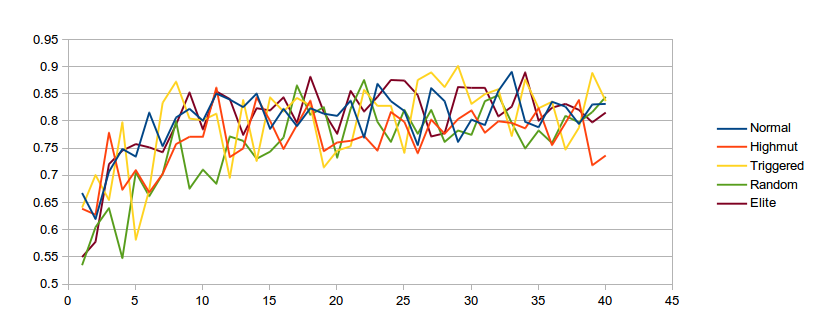
\includegraphics[width=\textwidth]{static.png}
 \caption[]   {Results on a static map.}
\label{fig:static}
\end{center}
\end{figure}

\begin{figure}[]
\begin{center}

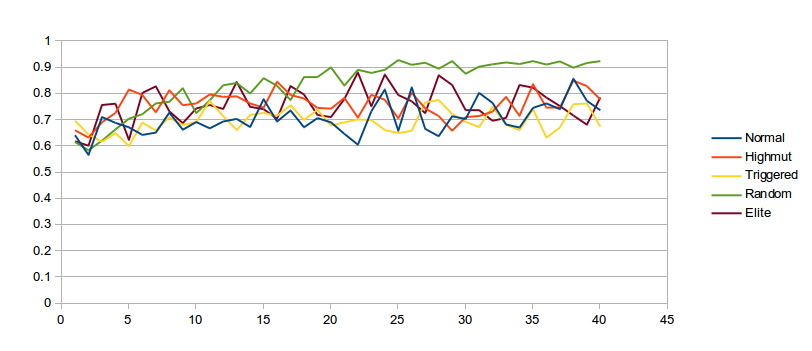
\includegraphics[width=\textwidth]{small.png}
 \caption[]   {Results on a slightly changing map.}
\label{fig:small}
\end{center}
\end{figure}

\begin{figure}[]
\begin{center}
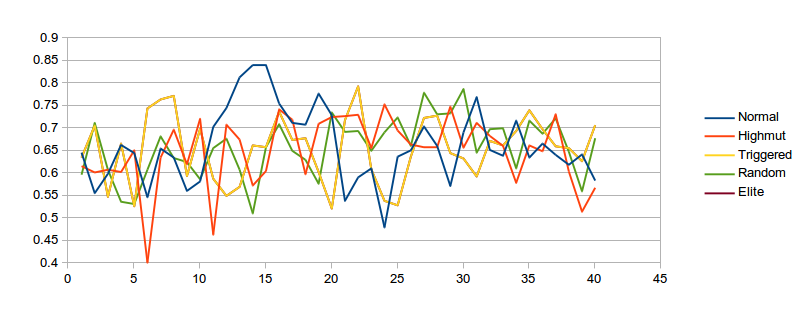
\includegraphics[width=\textwidth]{big.png}
 \caption[]   {Results on an abruptly changing map.}
\label{fig:big}
\end{center}
\end{figure}

\begin{figure}[]
\begin{center}
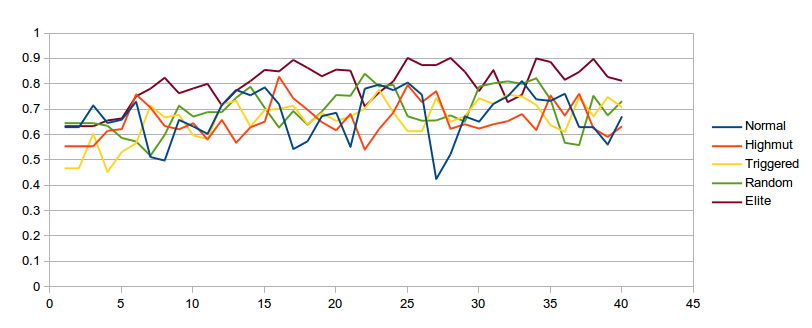
\includegraphics[width=\textwidth]{periodic.png}
 \caption[]  {Results on a periodically changing map.}
\label{fig:periodic}
\end{center}
\end{figure}



\section{Discussion}
\subsection{genome representation}
The genome is represented as an array of arrays. During a crossover (assuming 1-point crossover), the crossover will be row by row until the point of crossover, but could not be column by column. This means the convergence with this representation will be much more effective if the target (the food) lies in a horizontal line from their starting position, than if they lie in a vertical line. See figure \ref{fig:bias}.

\begin{figure}[h!]
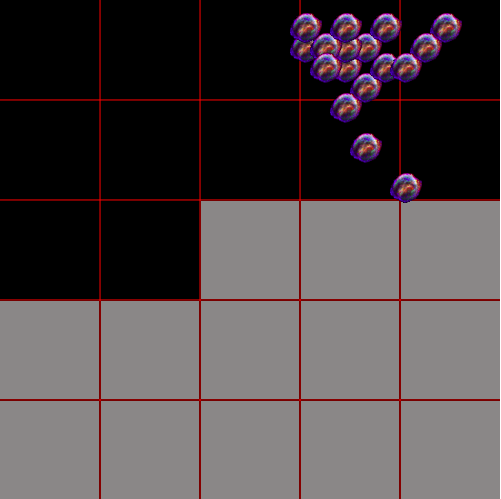
\includegraphics[width=0.4\textwidth]{TopRight.png}
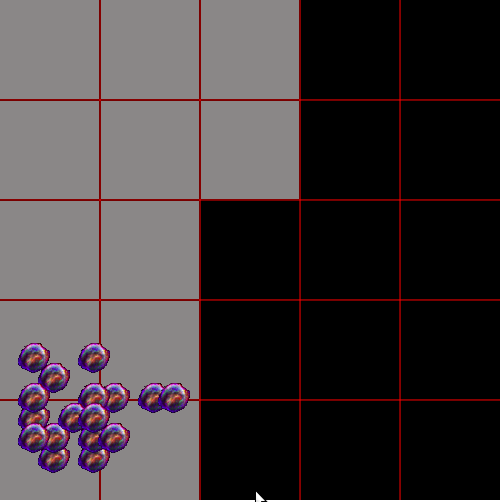
\includegraphics[width=0.4\textwidth]{BottomLeft.png}
\caption{The map in the left pictures is "easier" than the map in the right picture, even though one map is a rotation of the other. This is because the 1-point crossover illustrated to the left is possible with our representation of a genome, but the crossover to the right is not.}
\label{fig:bias}
\end{figure}

By randomly changing the starting position of the individuals at the start of each epoch, the impact of this bias can be lowered, as it is as as likely that the individuals will spawn with the food along a horizontal line from their position, as along a vertical line. Because of this problem of representation, uniform crossover was used consistently during testing as its bias is expected to be lower.

\subsection{Problem Difficulty}
In order to test the performance of the proposed dynamic methods, a graphical map was developed that provided the context in which evolution was taking place. In retrospect, this context proved to be far from optimal, mainly because of the difficulty of the problem. As can be seen in figure \ref{fig:static}, the algorithms do not converge even for a static environment, at the same time as the results for random behaviour is relatively high (never less that 0.5). This makes it difficult to know whether a higher fitness is due to random behaviour, or due to the nature of the method being run.

Another disadvantage was the dependency of the graphical interface. This requires significantly more processing power and time, making testing a time-consuming and cumbersome project. The results presented above were based on ten runs for each of the twenty combinations, which is a minimum number at best.

\subsection{Triggered Hypermutation}
The results obtained using triggered hypermutation did not display the results one would have expected. It is likely that this is due to the implementation, as the sources are not clear on the exact details. There are several parameters involved; i.e. ehen to enter the hypermutation phase, whether to decrease the mutation gradually or switching directly between high and low and how long the hypermutation phase should last. With this said, no conclusions are drawn about the effectiveness of this algorithm, based on the results obtained in this paper.

\section{Proposed Future Work}
We believe that the methodology used in this paper is suitable to reach the desired goal, but that the chosen environment could be improved. To further improve the results, a new environment and a new fitness function should be used to carry out the testing, in order to make the results more stable and more comparable. For the same reason, the number of tests could be significantly higher, although this would require more resources for testing.



\footnotesize
\begin{thebibliography}{4}
\bibitem{cobb}
H. G. Cobb, J. J. Grefenstette: Genetic Algorithms for Tracking Changing Environments. In: Proceedings of the 5th International Conference on Genetic Algorithms

\bibitem{simoes}
A. Simões, E. Costa: Using Genetic Algorithms to Deal with Dynamic Environments: A Comparative Study of Several Approaches Based on Promoting Diversity. In:  GECCO '02 Proceedings of the Genetic and Evolutionary Computation Conference

\bibitem{yang}
S. Yang: Genetic Algorithms with Elitism-Based Immigrants for Changing Optimization Problems. In: Lecture Notes In Computer Science, 2007, volume 4448, pages 627-636
\end{thebibliography}

\end{document}

